\documentclass[english, 12pt, a4paper, sci, utf8, a-2b, online]{aaltothesis}

%% DO NOT MOVE OR REMOVE \setupthesisfonts
\setupthesisfonts

%% Add here the packges you need
\usepackage{graphicx}
\usepackage{amsmath}
\usepackage{subcaption}


%% For tables that span multiple pages; used to split a paraphrasing example in
%% the appendix. If you don't need it, remove it.
\usepackage{longtable}

%% A package for generating Creative Commons copyright terms. If you don't use
%% the CC copyright terms, remove it, since otherwise undesired information may
%% be added to this document's metadata.
\usepackage[type={CC}, modifier={by-nc-sa}, version={4.0}]{doclicense}
%% Find below three examples for typesetting the CC license notice.


%% Edit to conform to your degree programme
%% Capitalise the words in the name of the degree programme: it's a name
\degreeprogram{Computer, Communication and Information Sciences}
\major{Macadamia}
% \major{Machine Learning, Data Science and Artificial Intelligence}
\univdegree{MSc}
\thesisauthor{Stefan Rua}

%% Your thesis title and possible subtitle comes here and possibly, again,
%% together with the Finnish or Swedish abstract. Do not hyphenate the title
%% (and subtitle), and avoid writing too long a title. Should LaTeX typeset a
%% long title (and/or subtitle) unsatisfactorily, you might have to force a
%% linebreak using the \\ control characters. In this case...
%% * Remember, the title should not be hyphenated!
%% * A possible 'and' in the title should not be the last word in the line; it
%%   begins the next line.
%% * Specify the title (and/or subtitle) again without the linebreak characters
%%   in the optional argument in box brackets. This is done because the title
%%   is part of the metadata in the pdf/a file, and the metadata cannot contain
%%   linebreaks.
\thesistitle{SAM2 pseudolabeling for instance segmentation}
\place{Espoo}
%% The date for the bachelor's thesis is the day it is presented
\date{30 September 2025}

%% Thesis supervisor
%% Note the "\" character in the title after the period and before the space
%% and the following character string.
%% This is because the period is not the end of a sentence after which a
%% slightly longer space follows, but what is desired is a regular interword
%% space.
\supervisor{Jorma Laaksonen}

%% Advisor(s)---two at the most---of the thesis. Check with your supervisor how
%% many official advisors you can have.
\advisor{Julius Pesonen (MSc)}

%% If you do your thesis work in a company of other institute, give the name of
%% the company or instution here. Otherwise, leave the macro empty, comment it
%% out, or remove it. This will remove this field from the abstract page.
\collaborativepartner{Finnish Geospatial Research Institute FGI}

%% Aaltologo: syntax:
%% \uselogo{?|!|''}
%% The logo language is set to be the same as the thesis language.
%%
\uselogo{?}
%\uselogo{!}
%\uselogo{''}
%%

%%%%%%%%%%%%%%%%%%               COPYRIGHT TEXT               %%%%%%%%%%%%%%%%%%
%%%%%%%%%%%%%%%%%%%%%%%%%%%%%%%%%%%%%%%%%%%%%%%%%%%%%%%%%%%%%%%%%%%%%%%%%%%%%%%%

%% Copyright of a work is with the creator/author of the work regardless of
%% whether the copyright mark is explicitly in the work or not. You may, if you
%% wish---we encourage you to do so---publish your work under a Creative
%% Commons license (see creativecommons.org), in which case the license text
%% must be visible in the work. Write here the copyright text you want using the
%% macro \copyrighttext, which writes the text into the metadata of the pdf file
%% as well.
%%
%% Syntax:
%% \copyrigthtext{metadata text}{text visible on the page}
%%
%% CHOOSE ONE OF THE COPYRIGHT NOTICE STYLES BELOW.
%% IF USING THE CC TERMS, CHOOSE THE LICENSE YOU WANT TO USE.
%% The different CC licenses are listed at 
%% https://creativecommons.org/about/cclicenses/.
%% If you use the icons from the dolicense.sty package, add the package above
%% (\usepackage{dolicense}).
%% IMPORTANT NOTE!! Manually write the CC text in the \copyrighttext metadata
%% text field.
%%
%% NOTE: In the macros below, the text written in the metadata must have a
%% \noexpand macro before the \copyright special character. When not in pdf/a
%% mode (i.e. a-1b or a-2b are not specified in \documentclass), two \noexpands
%% are required in the metadata text to correctly render the copyright mark in
%% the pdf metadata. In pdf/a mode one \noexpand suffices.
%%
%% EXAMPLE OF PLAIN COPYRIGHT TEXT
%% The macros \copyright and \year below must be separated by the \ character 
%% (space chacter) from the text that follows. The macros in the argument of the
%% \copyrighttext macro automatically insert the year and the author's name.
%% (Note! \ThesisAuthor is an internal macro of the aaltothesis.cls class file).
%%
%\copyrighttext{Copyright \noexpand\textcopyright\ \number\year\ \ThesisAuthor}
%{Copyright \textcopyright{} \number\year{} \ThesisAuthor}
%%
%% Of course, the same text could have simply been written as
%% \copyrighttext{Copyright \noexpand\copyright\ 2018 Eddie Engineer}
%% {Copyright \copyright{} 2022 Eddie Engineer}
%%
%% EXAMPLES OF CC LICENSE: different ways to display the same license
%% 1. A simple Creative Commons license text with a link to the copyright notice:
%\copyrighttext{\noexpand\textcopyright\ \number\year. This work is 
%	licensed under a CC BY-NC-SA 4.0 license.}{\textcopyright{} 
%	\number\year. This work is licensed under a 
%	\href{https://creativecommons.org/licenses/by-nc-nd/4.0/}{CC BY-NC-SA 4.0} 
%	license.}
%
%% To get the URL of the license of your choice, go to 
%% https://creativecommons.org/about/cclicenses/, click on the chosen license
%% you want to use, and copy-and-paste the URL in the macro \href above.
%%
%% 2. A short Creative Commons license text containing the respective CC icons
%% (requires the package dolicense.sty to be added in the preamble as done
%% above) and a link to the corresponding Creative Commons license webpage (see
%% the dolicense package documentation for other license icons):
%\copyrighttext{\noexpand\textcopyright\ \number\year. This work is licensed
%	under a CC BY-NC-SA 4.0 license.}{
%	\parbox{95mm}{\noindent\textcopyright\ \number\year. \doclicenseText} 
%	\hspace{1em}\parbox{35mm}{\doclicenseImage}
%}
%%
%% 3. An expanded Creative Commons license text containing the respective CC
%% icons text and as generated by the dolicense.sty package (the license is set
%% via package options in \usepackage[options]{dolicense} above; see the
%% dolicense package documentation for other license texts and icons):
\copyrighttext{\noexpand\textcopyright\ \number\year. This work is 
	licensed under a Creative Commons "Attribution-NonCommercial-ShareAlike 4.0 
	International" (BY-NC-SA 4.0) license.}{\noindent\textcopyright\ \number
	\year \ \doclicenseThis}
%%%%%%%%%%%%%%%%%%%%%%%%%%%%%%%%%%%%%%%%%%%%%%%%%%%%%%%%%%%%%%%%%%%%%%%%%%%%%%%%


%% The English abstract:
%% All the details (name, title, etc.) on the abstract page appear as specified
%% above.
%% Thesis keywords:
%% Note! The keywords are separated using the \spc macro
\keywords{pseudolabeling\spc instance segmentation\spc forestry}

%% The abstract text. This text in one paragraph is included in the metadata of
%% the pdf file as well as the abstract page. To have paragraphs in your
%% abstract rewrite it in the abstarct environment as described below.
\thesisabstract{
    Lorem ipsum etc.
}

%% You can prevent LaTeX from writing into the xmpdata file (it contains all the 
%% metadata to be written into the pdf file) by setting the writexmpdata switch
%% to 'false'. This allows you to write the metadata in the correct format
%% directly into the file thesistemplate.xmpdata.
%\setboolean{writexmpdatafile}{false}


%% All that is printed on paper starts here
%%
\begin{document}

%% Create the coverpage
%%
\makecoverpage

%% Typeset the copyright text.
%% If you wish, you may leave out the copyright text from the human-readable
%% page of the pdf file. This may seem like a attractive idea for the printed
%% document especially if "Copyright (c) yyyy Eddie Engineer" is the only text
%% on the page. However, the recommendation is to print this copyright text.
%%
\makecopyrightpage

\clearpage
%% Note that when writing your thesis in English, place the English abstract
%% first followed by the possible Finnish or Swedish abstract.

%% Abstract text
%% All the details (name, title, etc.) on the abstract page appear as specified
%% above. Add your abstarct text with paragraphs here to have paragraphs in the
%% visible abstract page. Nonetheless, write the abstarct text without
%% paragraphs in the macro \thesismacro so that it is added to the metadata as
%% well.
%%
\begin{abstractpage}[english]
    Lorem ipsum etc.
\end{abstractpage}

%% The text in the \thesisabstract macro is stored in the macro \abstractext, so
%% you can use the text metadata abstract directly as follows:
%%
%\begin{abstractpage}[english]
%	\abstracttext{}
%\end{abstractpage}

%% Force a new page so that the possible Finnish or Swedish abstract does not
%% begin on the same page
%%
\newpage
%%
%% Abstract in Finnish. Delete if you don't need it. 
%%
%% Respecify those fields that differ from the earlier specification or simply
%% respecify all fields.
\thesistitle{SAM2 pseudolabelöinti instanssisegmentaatiokoulutuksessa}
% \thesissubtitle{Opinnäytteen mahdollinen alaotsikko}
\supervisor{Jorma Laaksonen}
\advisor{DI Julius Pesonen}
\degreeprogram{Computer, Communication and Information Sciences}
\major{Macadamia}
\collaborativepartner{Paikkatietokeskus FGI}
\date{30.9.2025}
%% The keywords need not be separated by \spc now.
\keywords{pseudolabelöinti, instanssisegmentaatio, metsäily}
%% Abstract text
\begin{abstractpage}[finnish]
    Lorem ipsum jne.
\end{abstractpage}

\dothesispagenumbering{}

%% Table of contents. 
%%
\thesistableofcontents

%% Symbols and abbreviations
%\mysection{Symbols and abbreviations}
%\subsection*{Abbreviations}

\mysection{Abbreviations}

\begin{tabular}{ll}
ANN & artificial neural network \\
CHM & canopy height model \\
CNN & convolutional neural network \\
DSM & digital surface model \\
GSD & ground sample distance \\
IR & infrared \\
IoU & intersection over union \\
MLP & multilayer perceptron \\
NDVI & normalized difference vegetation index \\
NIR & near-infrared \\
R-CNN & region-based convolutional neural network \\
RPN & region proposal network \\
SAM & Segment Anything Model \\
SAM2 & Segment Anything Model 2 \\
mIoU & mean intersection over union \\
\end{tabular}

%% \clearpage is similar to \newpage, but it also flushes the floats (figures
%% and tables).
\cleardoublepage

\section{Introduction}
\label{sec:intro}

%% Leave page number of the first page empty
\thispagestyle{empty}

Airborne remote sensing based tree mapping methods are used for forest health monitoring \cite{ecke} and city planning \cite{velasquez} due to their efficiency compared to manual methods, but the training process is often bottlenecked by the need for high quality manual annotations. 
The goal of this thesis is to test if training results can be improved in instance segmentation tasks by refining coarse segments calculated from a canopy height model (CHM) using Segment Anything Model 2 (SAM2) \cite{sam2}.

In recent years, deep learning based methods have been shown to produce increasingly useful models and predictions in forestry and agriculture \cite{dl-forestry}, especially in the tasks of species detection and land cover prediction. Combined with the recent advances in autonomous data collection methods using unmanned aerial vehicles (UAVs) \cite{uav-data-collection}, there is unprecedented potential for massive data collection and mapping with relatively little manual labor. The efficient use of the available manual labor resources is especially important here in Finland where the population in small.

The ability to keep an up to date map of vegetation is essential for monitoring our forest ecosystems, which are increasingly important as global emissions rise and biodiversity decreases \cite{natural-resources-finland}. Finland has an especially great resposibility in protecting its nature, as an exceptionally large part of its surface area (75\%) is covered by forest. In addition to protecting boreal forests, efficiently managing areas used for by the forest industry is necessary, as it accounts for a significant part of the Finnish economy \cite{forest-industry-economy}. Finnish forests face unprecedented risks from bark beetles, drought, and forest fires due to climate change \cite{climate-change-finland-forestry}.

\subsection{Research Questions}

\begin{enumerate}
\item How much does SAM2 pseudolabeling improve low quality instance segmentation annotations?
\item How much does SAM2 pseudolabeling improve training results in instance segmentaion tasks?
\item How well does SAM2 pseudolabeling perform compared to other zero-shot instance segmentation methods?
\end{enumerate}

\subsection{Structure of the Thesis}

This thesis begins by explaining the necessary background information in the Backgroud section, and exploring the previous works relevant to this study in the Related Work section. The Dataset and Methods section contains a detailed explanation of the dataset, models, and training hyperparameters. Finally, the experiment's outcome is displayed and analyzed in the Results and Discussion sections, along with suggestions for future improvement.

\newpage
\section{Background}

This section goes over the necessary background information for understanding this thesis. Subsections explain the the machine learning task of instance segmentation, methods and model architectures to perform said task, the goals and methods of aerial tree mapping, and differences in remote sensing aerial imaging apparatus.

\subsection{Neural Networks}

Artificial neural networks (ANNs) are mathematical models, usually written as computer programs, designed to resemble the biological brain by imitating its structure of interconnected neurons. The goal of such models is to be "trained" using example data containing input and target pairs, after which the trained model is able to predict targets for new input data. The training is made possible by the interconnected neuron structure, represented as a graph where each neuron is a node, and each edge between nodes holds a tunable weight and bias parameter. The oldest and simplest type of neural network is the multilayer perceptron (MLP), that consists of an input layer of nodes, an output layer, and fully connected hidden layers in-between (Figure \ref{fig:mlp}). During training, the outputs of the model are compared to the ground truth targets and evaluated using a loss function. The gradients of the weights for each layer are calculated during the prediction phase called the forward pass, and updated based on the resulting loss during the backward pass. By repeating this backpropagation step over multiple iterations, the model's parameters gradually converge to predict the wanted targets for the given domain.
\cite{ann}

The gradient calculation and backpropagation step utilize the chain rule of differentiation: if $h = f(g(x))$, the derivative of $h(x)$, $h'(x)$ is

\begin{equation}
    h'(x) = f'(g(x))g'(x).
\end{equation}

\begin{figure}[h]
    \centering
    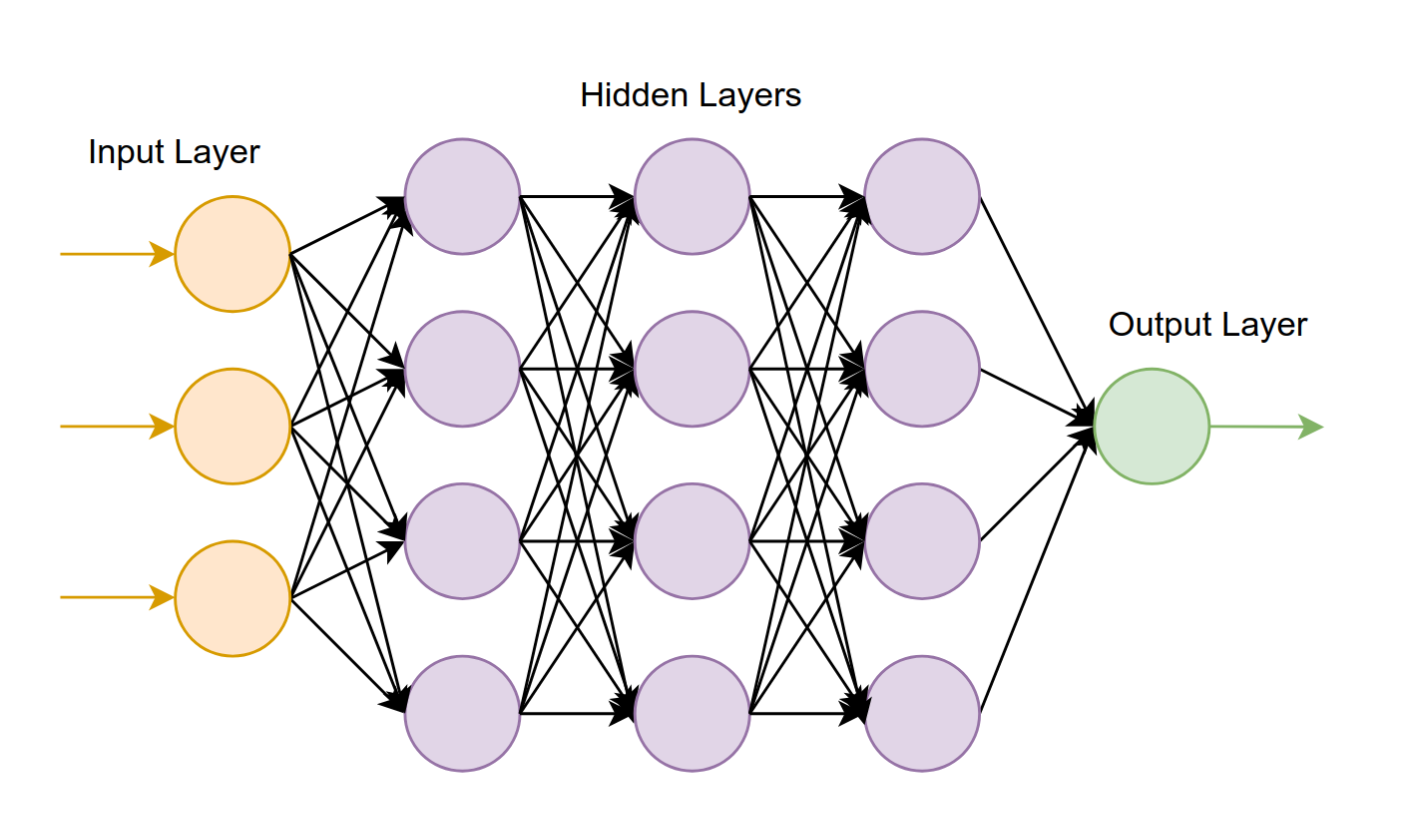
\includegraphics[width=0.7\textwidth]{figures/mlp.png}
    \caption{A multilayer perceptron visualized. \cite{julius}}
    \label{fig:mlp}
\end{figure}

\subsubsection{Convolutional Nerual Networks}

Convolutional neural networks (CNNs) are neural networks that employ convolutional layers. These are commonly used for computer vision tasks due to their efficiency in detecting hierarchies of visual features. A convolutional layer consists of a kernel that is moved over the input as a sliding window, computing an output for each position (Figure \ref{fig:convolutional}). The weights of the layer make up the kernel, and optimizing these weights lead to the kernel representing some feature related to the target. \cite{cnn}

\begin{figure}[h]
    \centering
    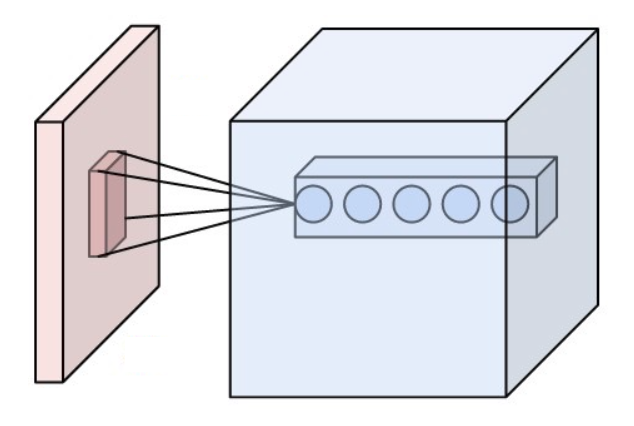
\includegraphics[width=0.5\textwidth]{figures/convolutional-layer.png}
    \caption{A convolutional layer visualized. \cite{convolutional-layer}}
    \label{fig:convolutional}
\end{figure}

\subsubsection{Transformers}

The transformer is a more recent neural network architecture that has shown great performance when trained on extremely large amounts of data. The network consists of an encoder that transforms the input into a set of tokens, that are then weighed using a self-attention layer, after which a decoder calculates the output based on the weighted tokens \cite{attention-is-all-you-need}. The main advantage of transformers is the ability to leverage massively parallel compute efficiently, allowing the training of very large models in a reasonable amount of time. An example of a transformer type neural network in shown in Figure \ref{fig:transformer}.

\begin{figure}[h]
    \centering
    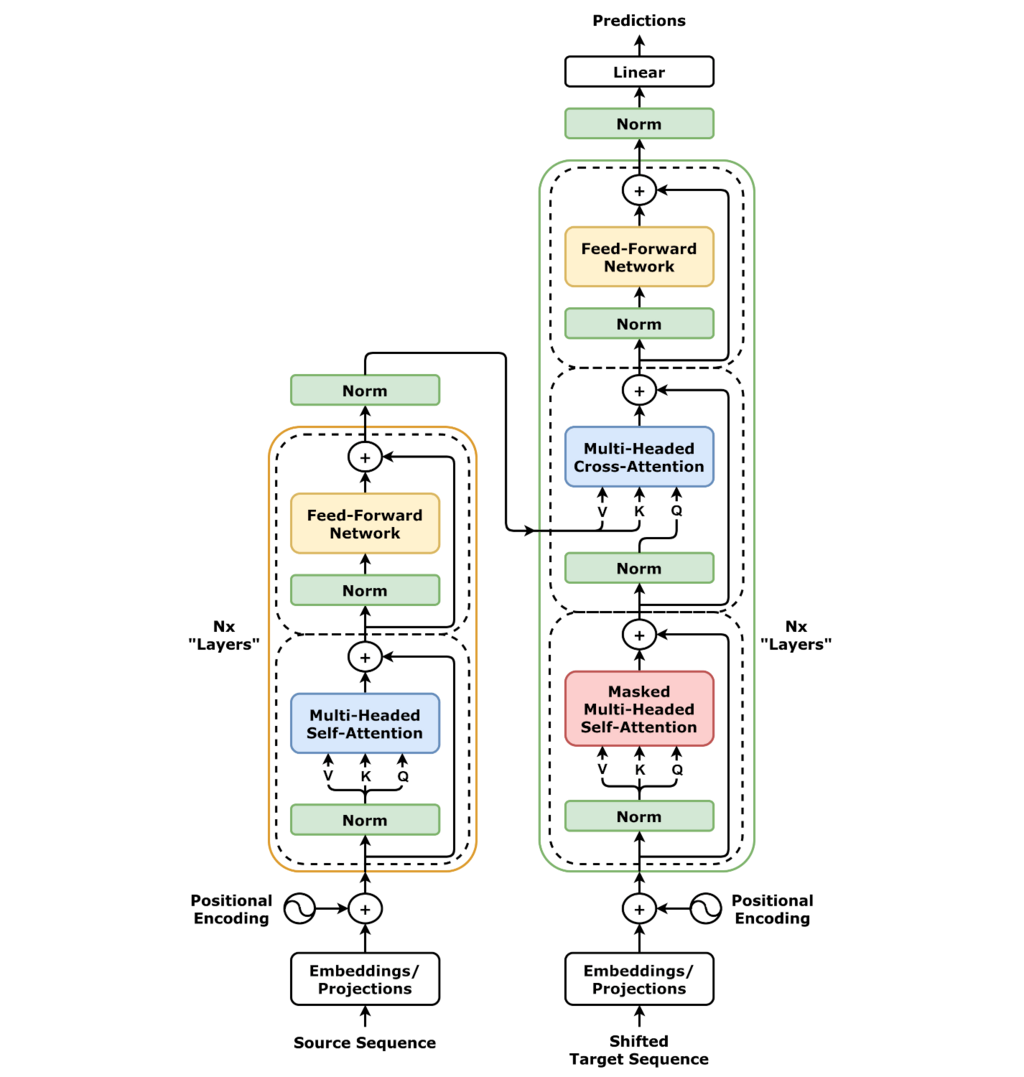
\includegraphics[width=0.7\textwidth]{figures/transformer.png}
    \caption{A transformer architecture visualized. Left: encoder, right: decoder. \cite{transformer}}
    \label{fig:transformer}
\end{figure}

\subsection{Instance Segmentation}

Instance segmentation is a machine learning task where the goal is to generate separate masks for individual objects in an image. This differs from semantic segmentation, where each pixel is given a semantic label without separating individual objects, and from object detection where individual objects are given bounding boxes but no masks. See Figure \ref{fig:task-comparison} for a visual comparison of the tasks.

\begin{figure}[h]
    \centering
    \begin{subfigure}[b]{0.32\textwidth}
        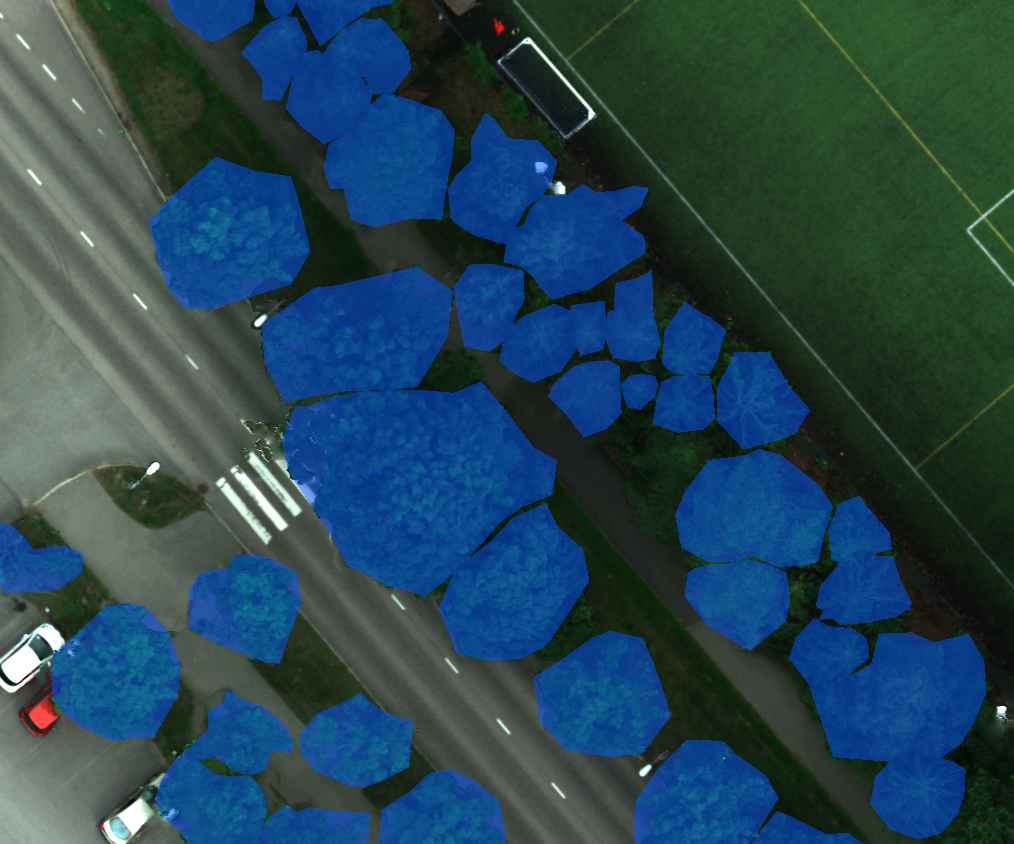
\includegraphics[width=1.0\textwidth]{figures/task-comparison/sem-seg.png}
        \caption{Semantic segmentation.}
    \end{subfigure}
    \begin{subfigure}[b]{0.32\textwidth}
        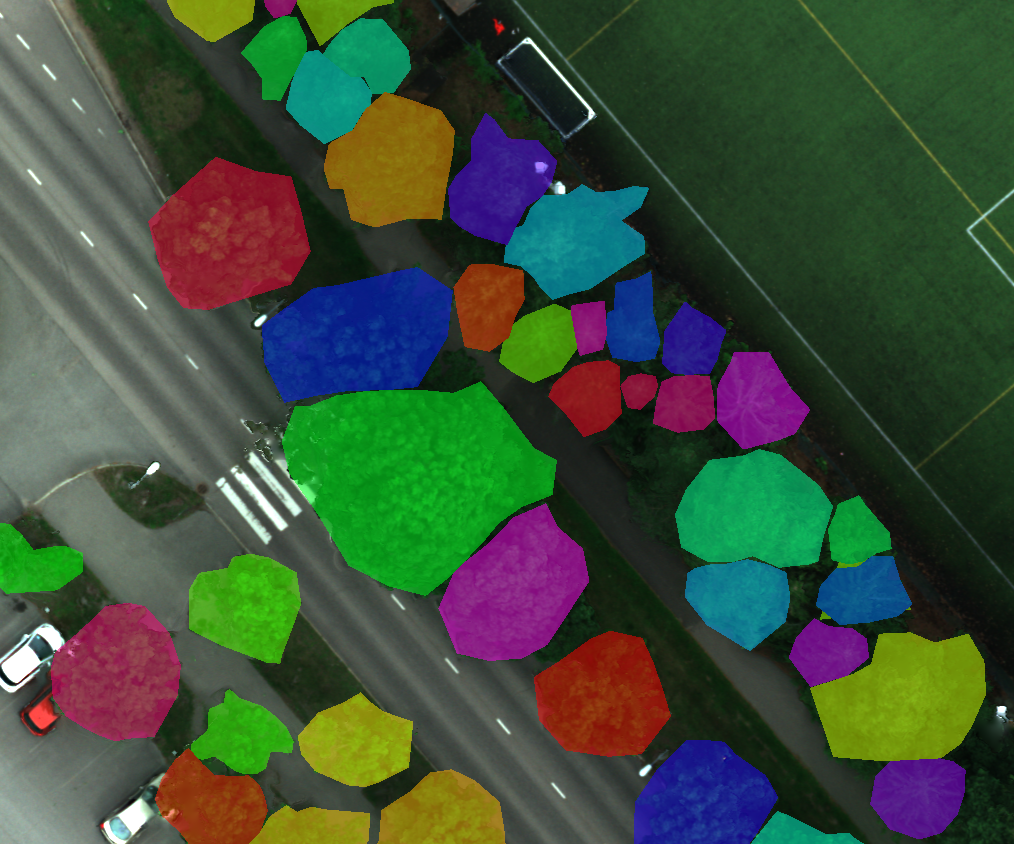
\includegraphics[width=1.0\textwidth]{figures/task-comparison/instance-seg.png}
        \caption{Instance segmentation.}
    \end{subfigure}
    \begin{subfigure}[b]{0.32\textwidth}
        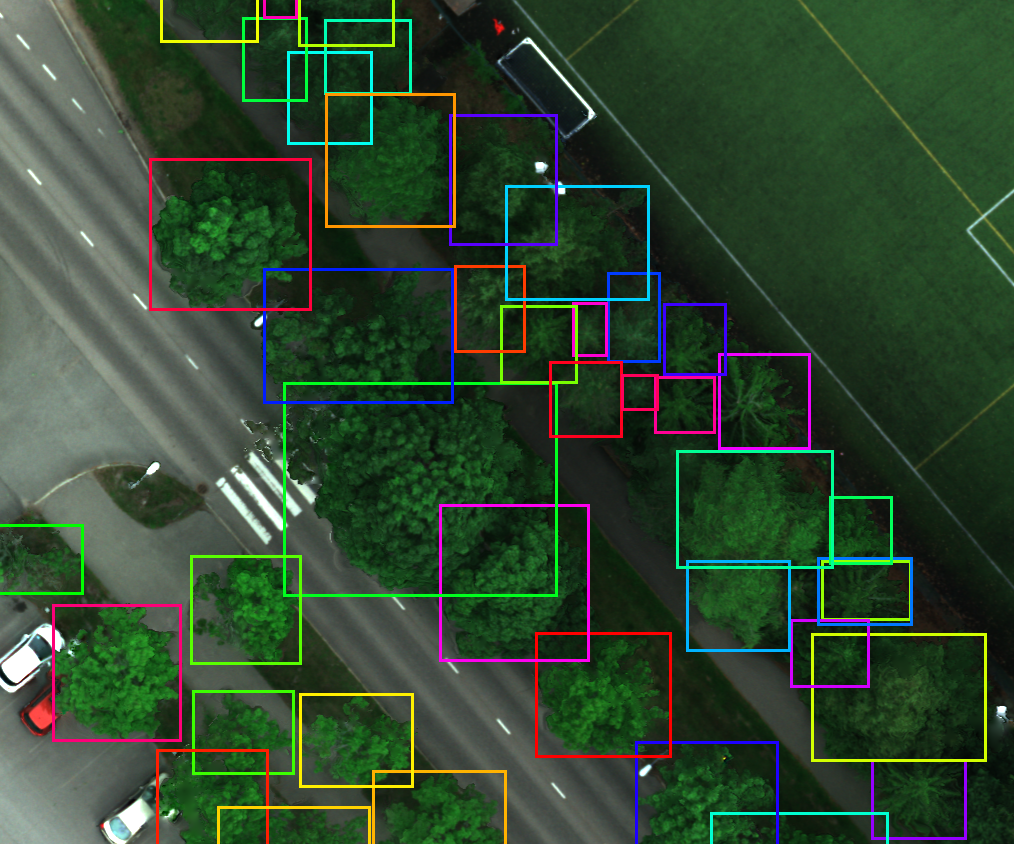
\includegraphics[width=1.0\textwidth]{figures/task-comparison/obj-det.png}
        \caption{Object detection.}
    \end{subfigure}
    \caption{Comparison of similar computer vision tasks.}
    \label{fig:task-comparison}
\end{figure}

\subsubsection{Mask R-CNN}

Mask R-CNN is an instance segmentation model based on a region-based convolutional neural network (R-CNN). It's trained using image-target pairs, where the target contains a binary mask, bounding box, and category label for each object of interest. After training, the model can predict masks in new images for the types of objects seen in training.

A CNN consists of convolutional layers, where the connections to the next layer are formed by sliding a kernel with tunable weights over the previous layer. R-CNNs search over feature maps produced by a CNN called the region proposal network (RPN) to find objects in images.

\subsubsection{Segment Anything Model 2}

Segment Anything Model 2 (SAM2) is a foundation model that can segment objects very generally, even ones that it hasn't been trained on. There are two ways to use it: only providing it with an image and letting it segment every object on its own, or providing it with an image and a prompt containing the location of the object of interest. The prompts can be of two types: a set of one or more foreground points and optional background points, or a bounding box (Figure \ref{fig:sam-prompts}). The model outputs a binary mask.

\begin{figure}[h]
    \centering
    \begin{subfigure}[t]{0.32\textwidth}
        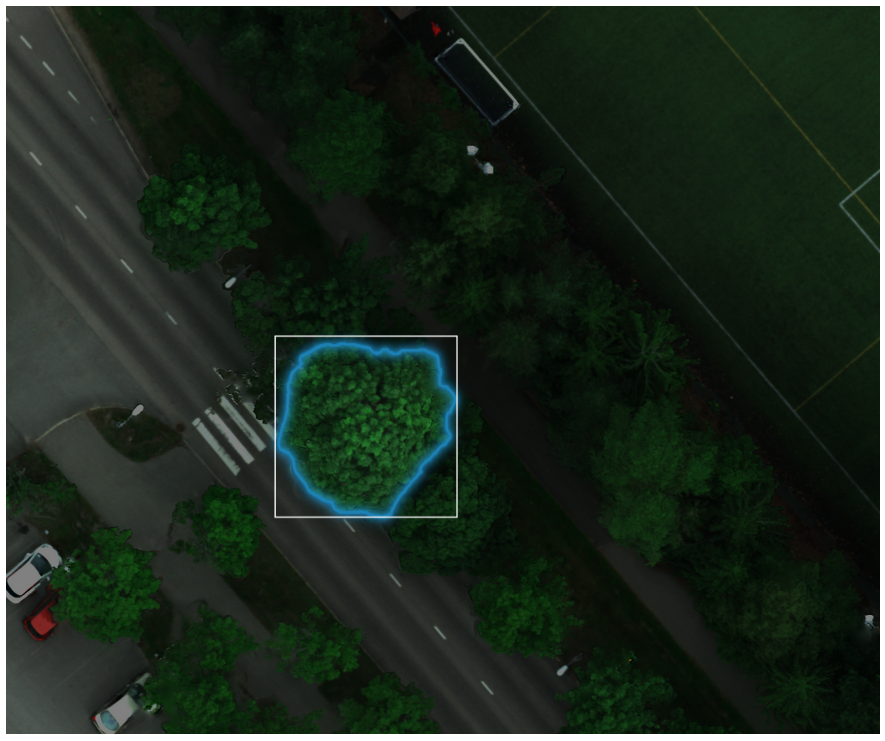
\includegraphics[width=1.0\textwidth]{figures/sam-prompts/box.png}
        \caption{Bounding box.}
    \end{subfigure}
    \begin{subfigure}[t]{0.32\textwidth}
        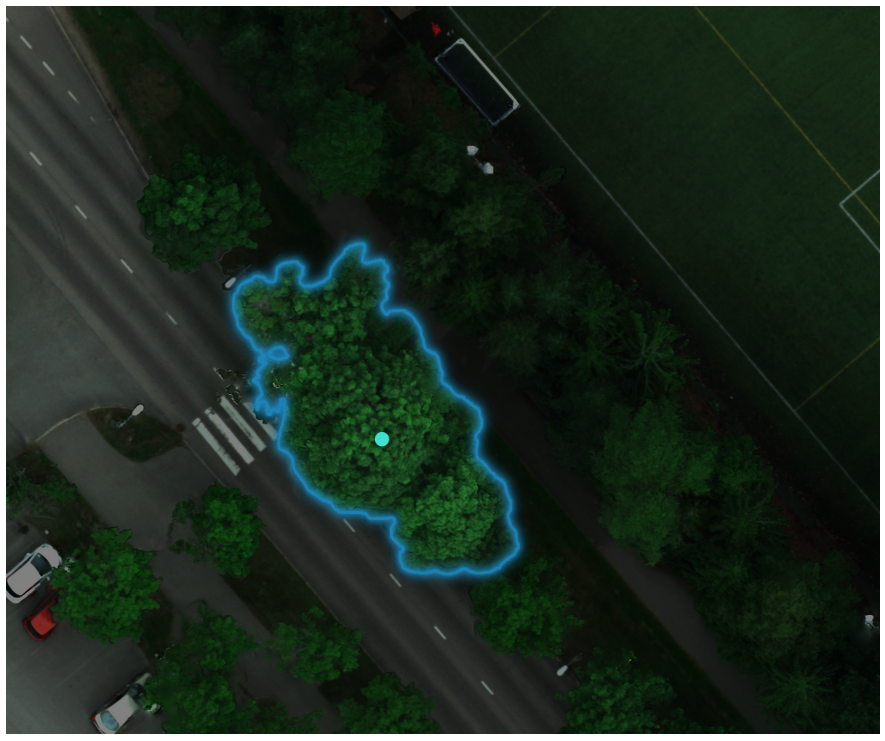
\includegraphics[width=1.0\textwidth]{figures/sam-prompts/point.png}
        \caption{Foreground point.}
    \end{subfigure}
    \begin{subfigure}[t]{0.32\textwidth}
        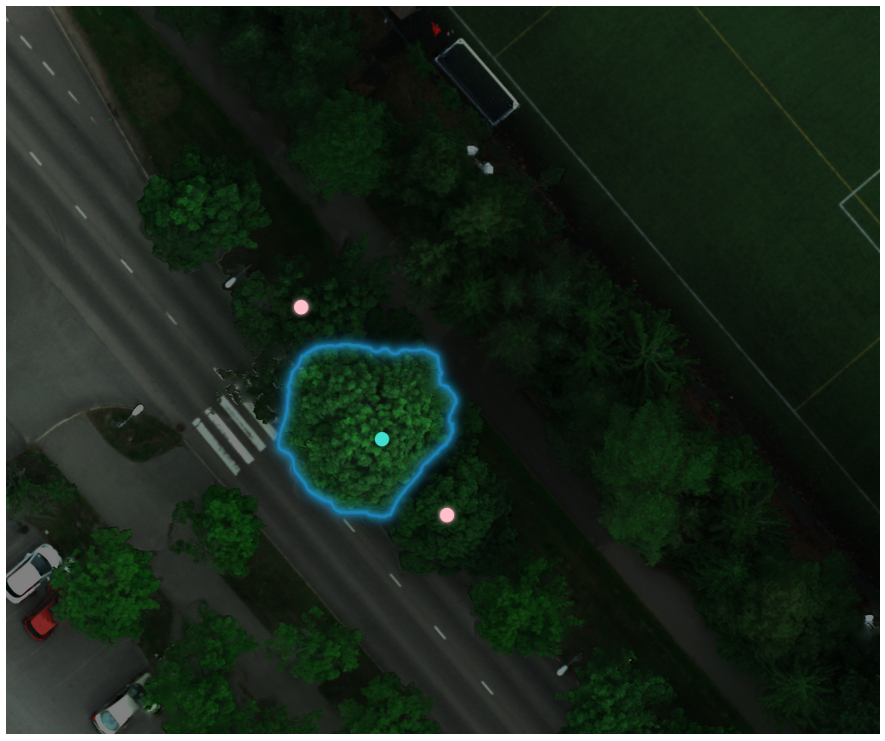
\includegraphics[width=1.0\textwidth]{figures/sam-prompts/point-background.png}
        \caption{Foreground and background points.}
    \end{subfigure}
    \caption{Comparison of SAM prompt types.}
    \label{fig:sam-prompts}
\end{figure}


SAM2 is a revised version of Segment Anything Model (SAM) \cite{sam}, a transformer-based foundation model for image segmentation. The main improvement in SAM2 the ability to train and predict on video data. While no video data was used in this thesis, SAM2 was chosen for its higher accuracy and 6x speedup over SAM.

\subsection{Aerial Tree Mapping}

Tree mapping is used by the forestry industry to monitor forest health, by urban planners to plan cities, by scientists to model ecological change and assess post-disaster damage.

Traditionally tree mapping has been done by ground-level visual analysis \cite{aerial-photography}, but the advent of aerial photography, laser scanning, and computational analysis has moved this task towards remote sensing.

\subsubsection{Aerial Imaging}

Aerial images may be taken from any airborne apparatus, for example drones, helicopters, aeroplanes, or even satellites. For the purpose of mapping individual trees satellite imagery rarely provides a high enough ground sample distance (GSD), and aeroplanes aren't convenient for covering square-ish areas, so drones and helicopters are most often used.

\begin{figure}[h]
    \centering
    \includegraphics[width=0.7\textwidth]{figures/drone.jpg}
    \caption{Drone with remote sensing apparatus.}
    \label{fig:drone}
\end{figure}

Aerial remote sensing sensors include laser scanners and multispectral cameras in addition to traditional RGB-cameras that only capture visible wavelengths. Laser scanners produce three-dimensional point could data. Point clouds be used for volumetric segmentation or detection, or for calculating a digital surface model (DSM) or canopy height model (CHM). A DSM models the surface of the ground and protruding objects, and a CHM models the height the tree canopy.
\newline
\newline
[image of point cloud, image of dsm]
\newline

Multispectral cameras can capture additional wavelengths invisible to the human eye. Typically these include infrared (IR) at 1550-1750 nm and near-infrared (NIR) at 750-900 nm. Hyperspectral cameras capture a continuous spectrum instead of discrete channels. In forestry and agriculture, this extended range of bandwidths can provide useful information for biomass and growth stage estimation and species detection. \cite{hyperspectral-agricultural}
\newline
\newline
[hyperspectral graph]
\newline

\newpage
\section{Related Work}

The previous version of SAM2, SAM has been assessed for tree crown instance segmentation on drone imagery \cite{sam-treecrown}. The study uses SAM in the following ways: generating masks without any prompts, generating masks with digital surface model (DSM) maxima as point prompts, and prompting SAM with predictions from a trained Mask R-CNN model. Of these, the last approach is closest to the one examined here. The resulting mean intersection over union (mIoU) scores the single-class detection class were as follows: SAM + no prompts: 35.06\%, SAM + DSM prompts: 46.15\%, Mask R-CNN + SAM: 78.27\%.

Another study examining SAM for remote sensing use proposes RSPrompter \cite{rsprompter}, a method that learns to generate prompts from the SAM's image encoder, then feeding them to the decoder. The study proposing the method reports the results as AP scores, but the study mentioned above tested RSPrompter as well, achieving 82.58\% mIoU. \cite{sam-treecrown}

FMARS \cite{fmars} is a dataset with annotations generated using GroundingDINO and SAM. GroundingDINO was used to convert text prompts to bounding boxes, and SAM for converting these boxes to segments. A subset of the annotated area was manually annotated, and the generated annotations were compared to the manual ones, resulting in a mIoU score of 50.22\%.

\newpage
\section{Dataset and Methods}

This section covers the technical details of the dataset and methods used to train and evaluate the models.

\subsection{Dataset}

The main dataset consists of a multispectral orthophoto taken from Espoonlahti by helicopter spanning approximately 2 km$^2$ (Figures \ref{fig:dataset-ortho} and \ref{fig:dataset-test}) and CHM-based coarse tree crown segments. The orthophoto covers both forest and urban area, has a GSD of 2.5 cm, and contains blue, green, red, near-infrared, mid-infrared, and thermal infrared bands.

\begin{figure}[h]
    \centering
    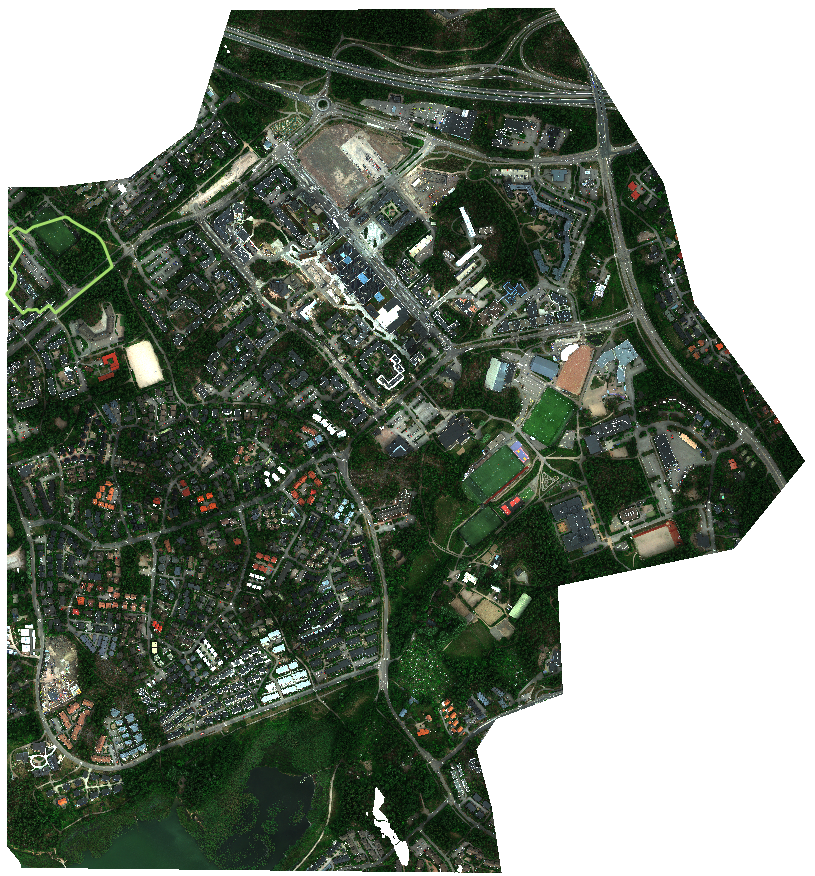
\includegraphics[width=0.6\textwidth]{figures/dataset-ortho.png}
    \caption{Dataset (RGB channels shown). The test area is delineated in green.}
    \label{fig:dataset-ortho}
\end{figure}

\begin{figure}[h]
    \centering
    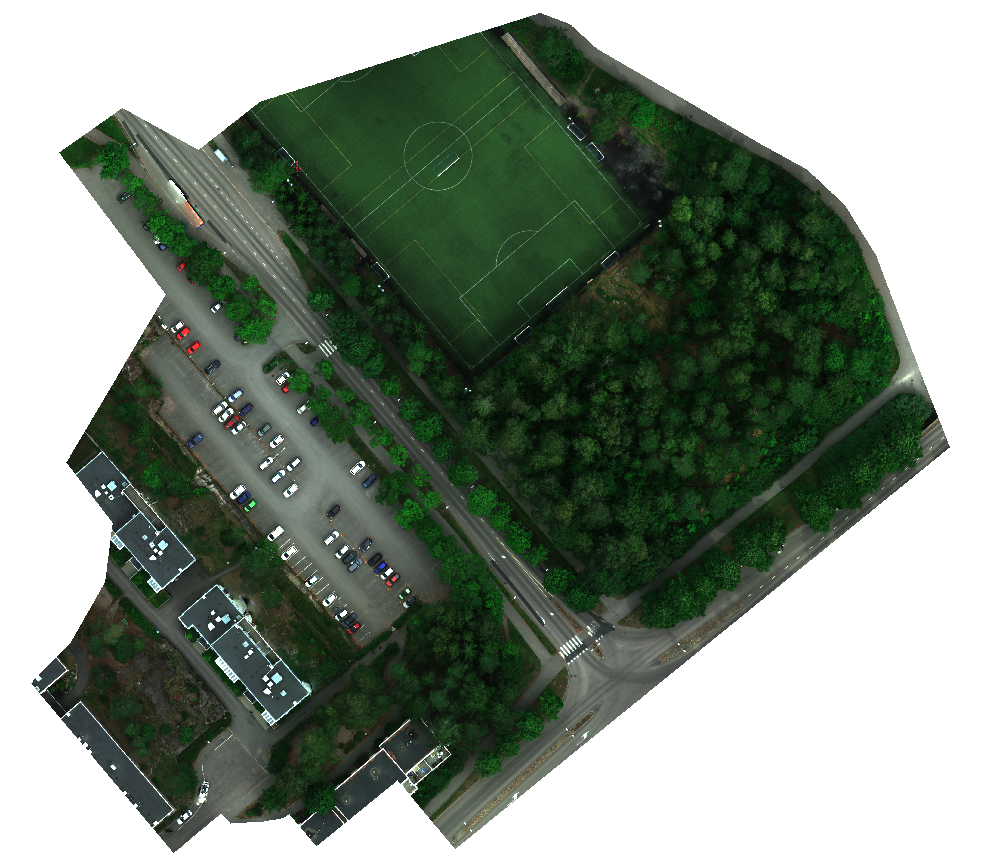
\includegraphics[width=0.6\textwidth]{figures/dataset-test.png}
    \caption{The test area (RGB channels shown).}
    \label{fig:dataset-test}
\end{figure}

As the CHM-based coarse tree crown segments had been calculated from point-cloud data from an earlier flight than the multispectral images, many segments no longer contained trees. To eliminate these erroneus segments, they were filtered based on their Normalized Difference Vegetation Index (NDVI) value:

\begin{equation}
\text{NDVI} = \frac{\text{NIR - Red}}{\text{NIR + Red}}.
\end{equation}

For each segment, NDVI was calculated using the per-channel mean values. Segments with NDVI < 0.2 were removed. Figure \ref{fig:ndvi} shows the distribution of NDVI values.

\begin{figure}[h]
    \centering
    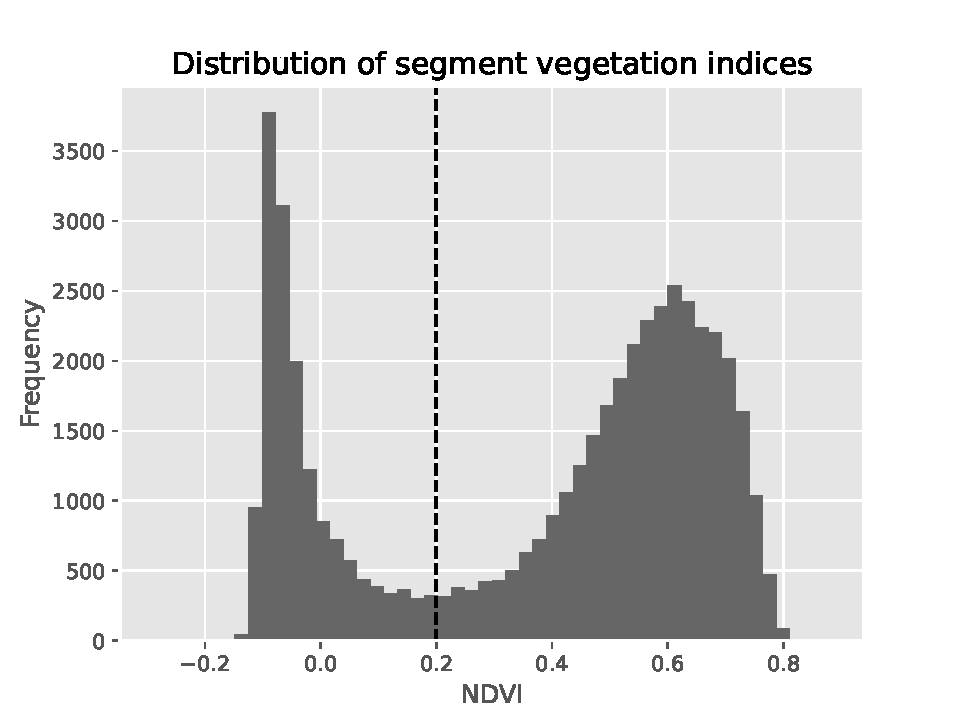
\includegraphics[width=0.7\textwidth]{figures/ndvi.pdf}
    \caption{Distribution of NDVI values. The dashed vertical line indicates the threshold below which segments were discarded.}
    \label{fig:ndvi}
\end{figure}

\subsection{Models}

SAM2 is used for the pseudolabeling task and Mask R-CNN \cite{maskrcnn} for the supervised instance segmentation.

\subsection{Methods}

First the coarse segments were pseudolabeled using SAM2, indexing the orthphoto in a grid with a window of size 1024 and a stride of 512. For each window, only the segments whose centroids were located in the central 512x512 square of the window were selected for pseudolabeling. Then, the bounding box of each segment was passed as a prompt to SAM2, and the largest connected component of the output mask was saved as the pseudolabel. These parameters for the window size and stride were selected in order to avoid stitching artifacts and to provide SAM2 with images matching the native input resolution of the model. An example of the pseudolabeling process is shown in Figure \ref{fig:pseudolabel}, and the distribution of tree radii is shown in Figure \ref{fig:radii}.

\begin{figure}[h]
    \centering
    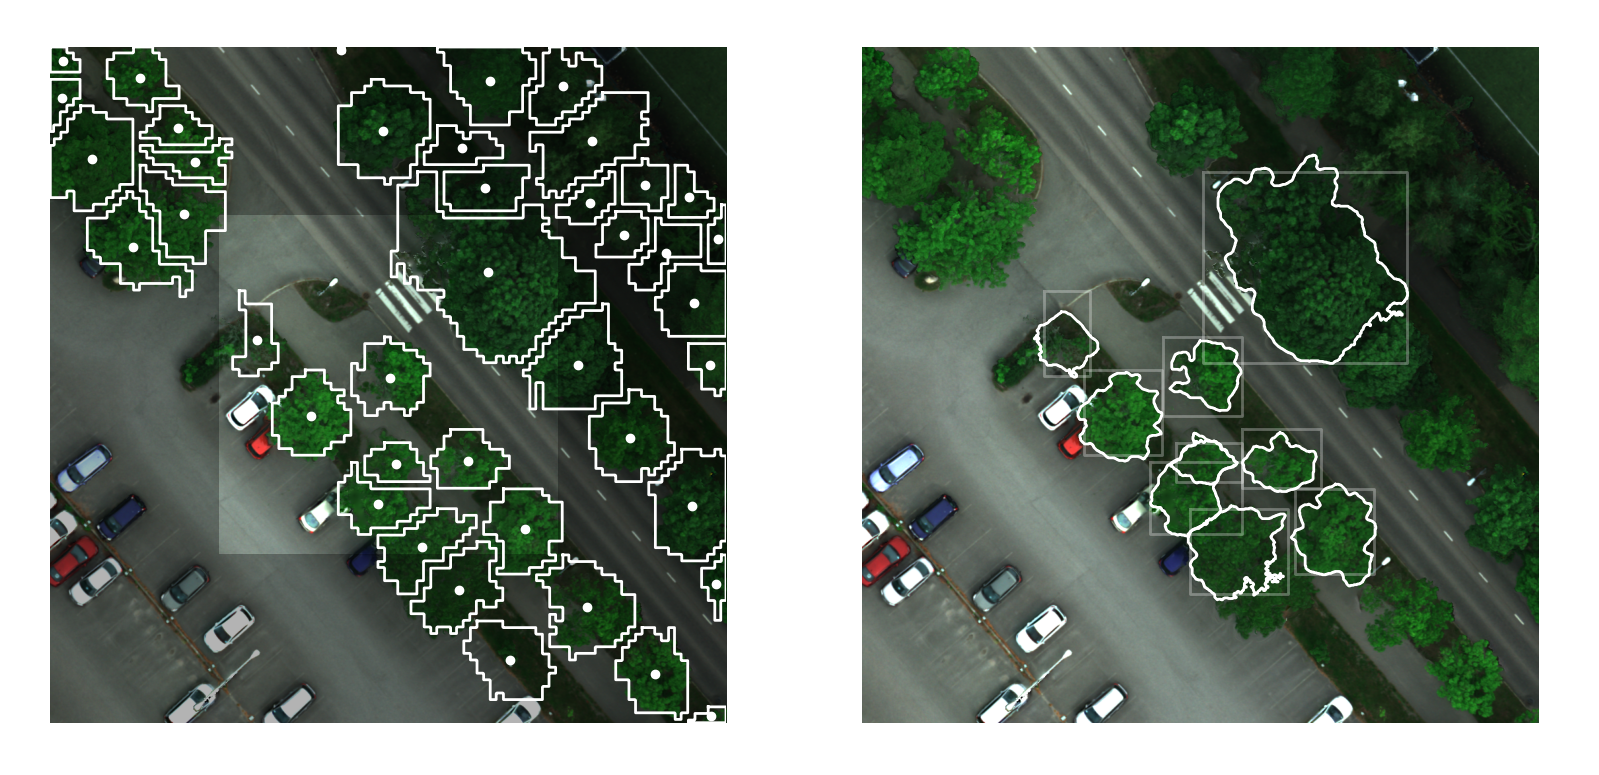
\includegraphics[width=1.0\textwidth]{figures/pseudolabel1.png}
    \caption{Example of the pseudolabeling process. On the left, CHM-based coarse segments are drawn around tree crowns, and their centroids are displayed as dots. The shaded area around the central 512x512 square is the buffer region. On the right, the box prompts provided to SAM are shown in reduced opacity, and the predicted mask outlines are drawn in white.}
    \label{fig:pseudolabel}
\end{figure}

\begin{figure}[h]
    \centering
    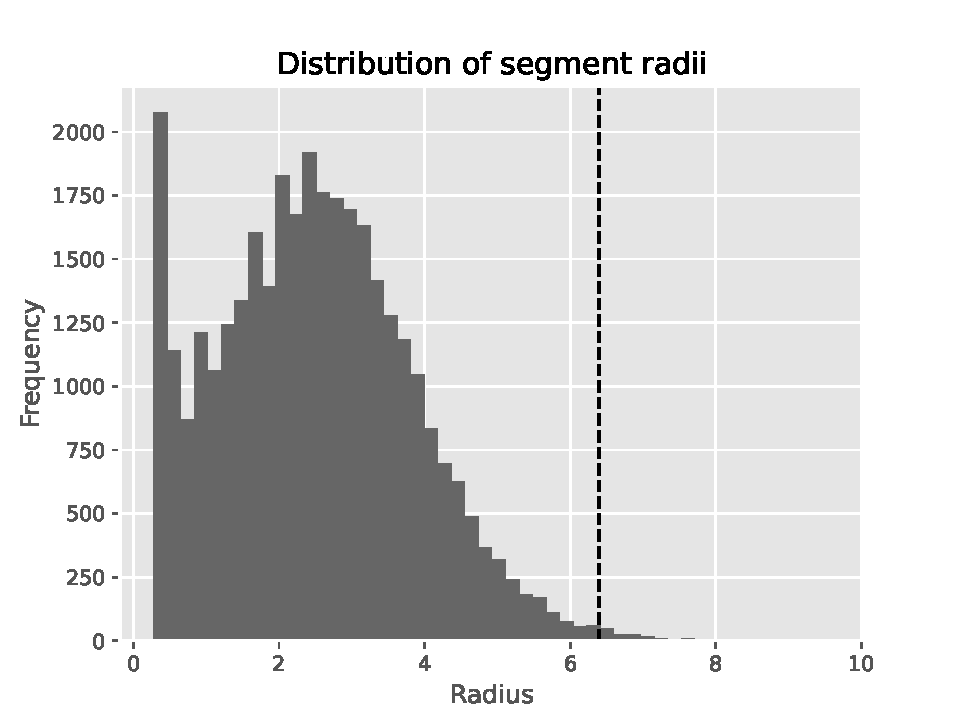
\includegraphics[width=0.7\textwidth]{figures/radii.pdf}
    \caption{Distribution of tree crown radii. The dashed vertical line indicates the threshold above which segments may span from the central region of interest over the buffer region to the image border, producing stitching artifacts.}
    \label{fig:radii}
\end{figure}

A small test area of 362 trees was segmented manually. To evaluate the quality of the coarse segments and quantify the effect of SAM2 pseudolabeling, the coarse segments and pseudolabels were compared to the manual segments using the Jaccard index. Figure \ref{fig:annotation-comparison} shows the visual differences between the original coarse CHM-based segments, pseudolabels produced by SAM, and manually drawn segments.

\begin{figure}[h]
    \centering
    \begin{subfigure}[b]{0.32\textwidth}
        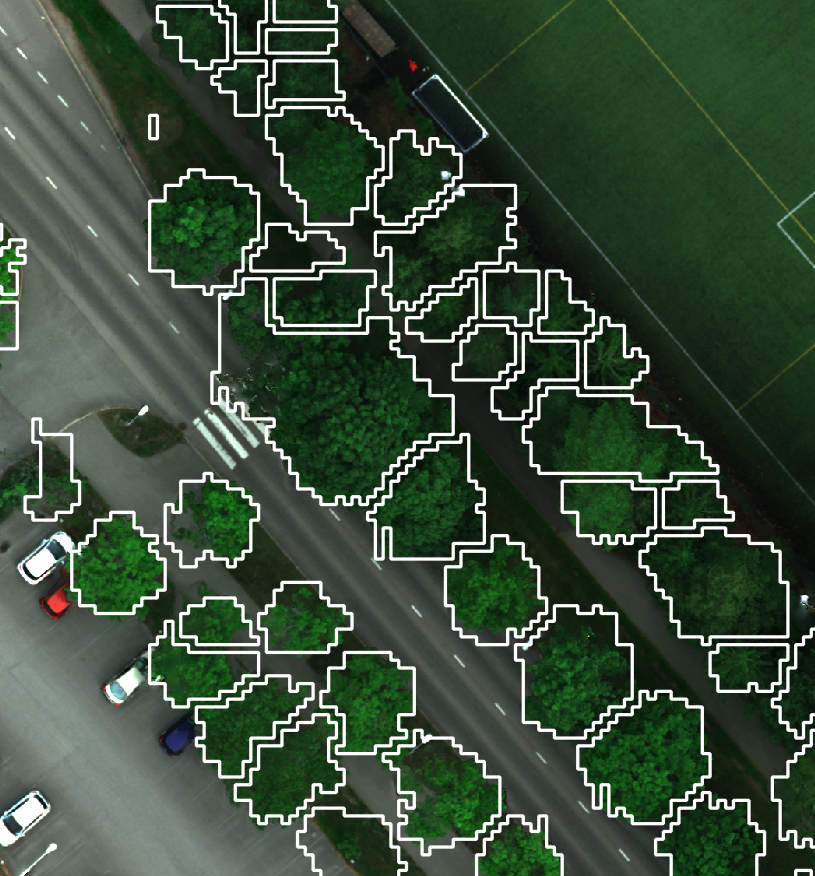
\includegraphics[width=1.0\textwidth]{figures/annotations/coarse.png}
        \caption{Coarse, CHM-based.}
    \end{subfigure}
    \begin{subfigure}[b]{0.32\textwidth}
        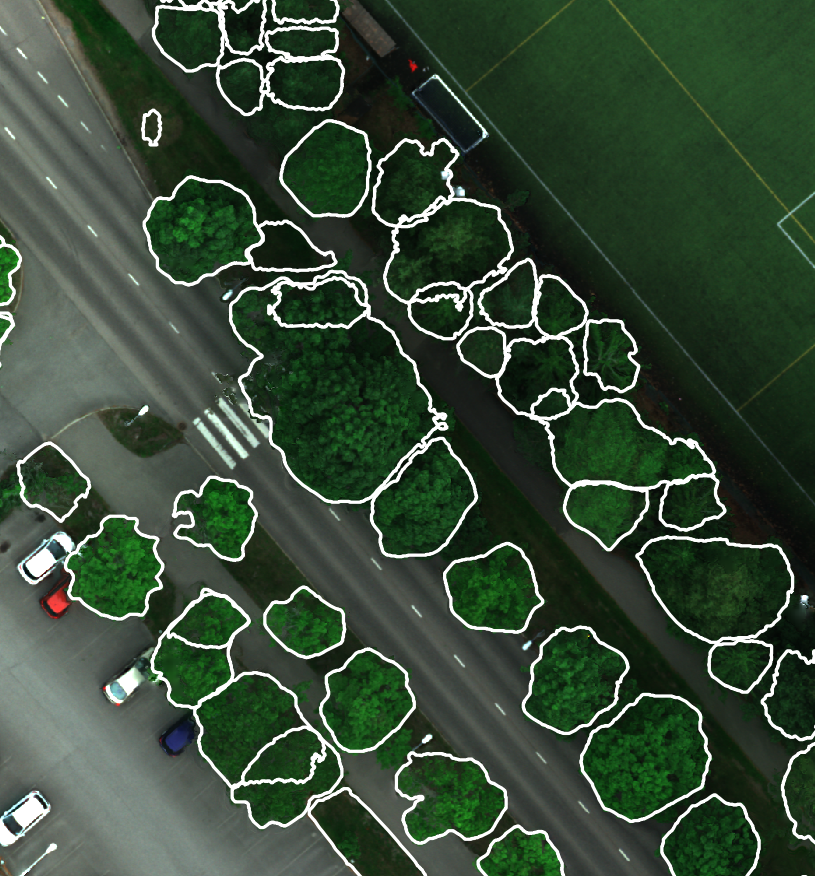
\includegraphics[width=1.0\textwidth]{figures/annotations/pseudolabeled.png}
        \caption{SAM pseudolabels.}
    \end{subfigure}
    \begin{subfigure}[b]{0.32\textwidth}
        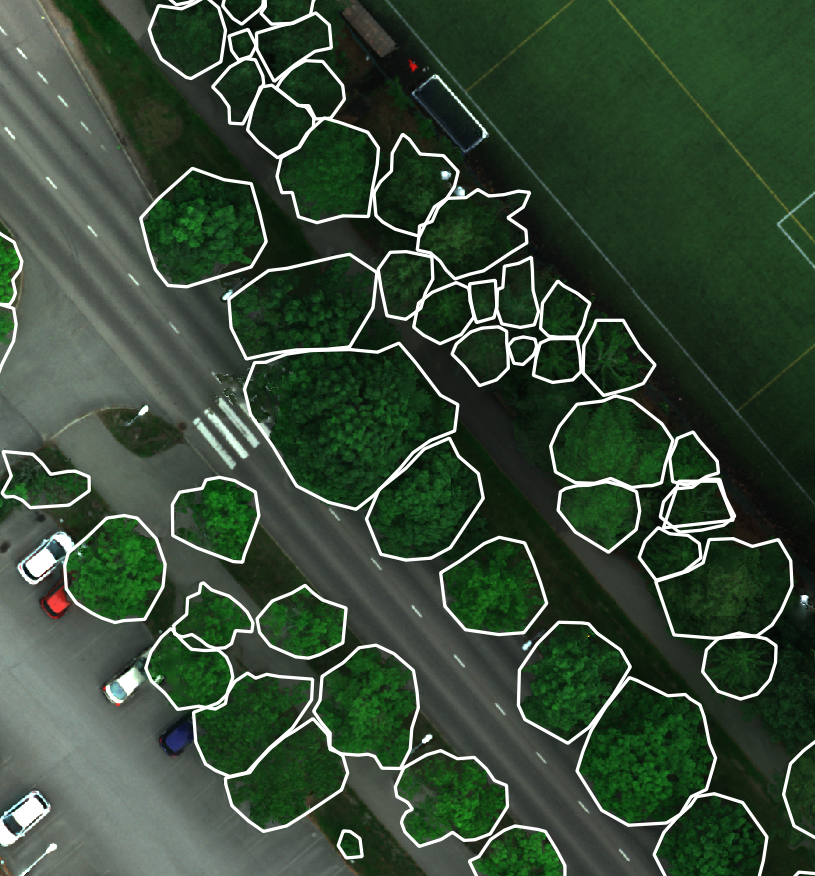
\includegraphics[width=1.0\textwidth]{figures/annotations/manual.png}
        \caption{Manual.}
    \end{subfigure}
    \caption{Comparison of annotations.}
    \label{fig:annotation-comparison}
\end{figure}

Then, a Mask R-CNN model with a ResNet-50 \cite{resnet} backbone was trained separately on both the coarse segments and pseudolabels. The optimizer was AdamW \cite{adamw} with a learning rate of 1e-6 and weight decay of 1e-2.

\newpage


\subsection{Performance Measures}

\subsubsection{Jaccard Index}

The Jaccard index\cite{jaccard} is a measure of similarity between two segments:

\begin{equation}
J(A, B) = \frac{|A \cap B|}{|A \cup B |},
\end{equation}

where A and B are the segments to be compared. This performance measure is also referred to as IoU (intersection over union), and utilized in the mIoU metric, the mean of IoU-scores over all target classes.

\subsubsection{Precision and Recall}

Precision and recall meaure the quality of a model's predictions. Precision is the fraction of detections that truly contained a target:

\begin{equation}
    \text{Precision} = \frac{\text{Correct detections}}{\text{All detections}}, 
\end{equation}

and recall is the fraction of targets that were detected:

\begin{equation}
    \text{Recall} = \frac{\text{Detected targets}}{\text{All targets}}.
\end{equation}

\subsubsection{$F_1$ score}

The $F_1$ score is a performance measure that represents the overall performance of a model as the harmonic mean of precision and recall:

\begin{equation}
    F_1 = \frac{2}{\text{recall}^{-1} + \text{precision}^{-1}}.
\end{equation}


\section{Experiments and Results}

(Results table with accuracy, recall, f1, and miou for each model here)

The highest scoring model was ???. The addition of the SAM2 pseudolabeling preprocessing step improved accuracy by ??\%, recall by ??\%, F1 by ??\%, and mIoU by ??\%.

\subsection{Discussion}

The segmentation performance improvement provided by pseudolabeling indicates that it is a worthwhile preprocessing step for datasets, where the original annotations are only approximate.

\section{Conclusions}

\clearpage

\thesisbibliography
\bibliographystyle{IEEEtran}
\bibliography{references}

\end{document}
